\documentclass[]{article}
\usepackage[UTF8]{ctex}
\usepackage{graphicx}
\usepackage{amsmath}
\usepackage{amsfonts}
\newtheorem{definition}{Definition}
\newtheorem{theorem}{Theorem}
\newtheorem{proposition}{Proposition}
\newtheorem{lemma}{Lemma}

%opening
\title{对称加密的一种具体安全处理\footnote{原文:M. Bellare, A. Desai, E. Jokipii and P. Rogaway, "A concrete security treatment of symmetric encryption," Proceedings 38th Annual Symposium on Foundations of Computer Science, 1997, pp. 394-403, doi: 10.1109/SFCS.1997.646128.}}
\author{作者:M. Bellare,A. Desai,E. Jokipii,P. Rogaway\\
\small{译者:李晓峰,北京联合大学智慧城市学院\footnote{译者email:cy\_lxf@163.com,译文来自于译者发起的“信息安全经典翻译”开源项目https://gitee.com/uisu/InfSecClaT}}
}


\usepackage{hyperref} %生产书签

\begin{document}

\maketitle

%\tableofcontents %生产目录

\begin{abstract}
我们在具体安全(concrete security)框架内研究对称(如私钥)加密方案的概念。\par
我们给出四种不同的抵抗选择明文攻击(chosen plaintext attack)的安全概念,分析这些概念之间规约的具体复杂度,提出了上下限,并获得了这些概念间的紧密关系。利用这样的方法,我们对概念根据在具体安全方面更强或更弱进行了分类(尽管相互间可以多项式规约)。\par
接下来我们提供了分组密码加密方法的具体安全性分析,包括最流行的加密方法CBC,我们将对手模型化为他们的资源函数,从而建立了严格的界限(意味着匹配上界和攻击)。
\end{abstract}

\section{引言}
加密方案使Alice能够以这样的方式向Bob发送消息,即敌方Eve不会获得关于消息内容的重要信息。这是密码学的经典问题。通常在两种设置(setting)中考虑。在对称(私钥)系统中,加密和解密是在发送方和接收方共享的密钥下执行的。在非对称(公钥)设置中,发送方具有一些公共信息,接收方持有一些相应的秘密信息。\par

在本文中,我们有两个目标。第一个是在具体安全框架中研究对称加密的概念。这意味着我们将研究不同概念之间规约的具体复杂性。我们想证明上下界。通过这种方式,我们可以在概念之间建立紧密的关系,并可以比较概念(即使彼此可多项式规约)的强弱。\par

第二个目标是提供一些特定对称加密方案的具体安全性分析。我们考虑的其中一种方案(CBC加密)是普遍使用的,但在传统可证明安全性中从未进行形式化分析(具体或其他)。我们想纠正这一点。同样,目标是找到对手成功概率的严格界限,作为其消耗资源的函数,这包括证明上界和匹配下界。

\subsection{背景和动机}
Goldwasser和Micali的开创性工作[11]是第一个为加密引入安全的形式化概念。具体来说,他们提出了非对称加密的两个安全概念,“语义安全”和“多项式安全”,并证明了它们在多项式时间规约方面是等价的。Micali、Rackoff和Sloan[17]表明,这些概念的(适当版本)也等同于姚[20]提出的另一个概念。Goldreich[8]给出了非对称加密概念的统一复杂性处理。Luby[15,第11-12章]提出了这些概念对对称设置的一些修改。
\par

Goldwasser和Micali[11]还提出了一种非对称加密方案,其安全性(在上述意义上)是可从二次剩余多项式时间规约。随后,基于各种难题,出现了许多其他方案。\par

\textbf{{\large 具体安全(concrete security).}}
上述所有工作的观点是,如果两个安全概念之间存在多项式时间规约,则它们是等价的;并且如果从一个困难问题到一个方案存在多项式时间规约,则该方案被声明为可证明安全的。这些当然是基本问题,但我们认为,一旦知道答案,就必须以更精确的方式对概念和方案进行分类。\par

打个比方,只关心密码学中的多项式时间可规约有点像只关心计算问题是否在P中。然而,我们知道有许多有趣的问题(包括算法领域的大部分,以及复杂性理论)围绕着获取已知在P中的问题的进一步信息。这些信息有助于更好地理解问题,对于实际应用也是必不可少的。\footnote{译者注:打比方是为了用一个大家都知道的东西做类比,编译理解新的问题或较难的问题,Bellare是学数学出身,估计他认为大家应该对计算复杂性都有了解,所以用这个打比方。}
\par

在密码学中,多项式等价概念的具体复杂性情况类似。特别是,当规约不是保持安全(security-preserving)时,这意味着必须使用更大的安全参数才能安全,从而降低效率。因此,最终,我们为低效规约在保证或运行时间方面付出了代价。\par

我们的具体安全方法是[5,6]的方法,其中一种方法参数化了所涉及的资源,并通过其上\footnote{译者注:这里的“其上”是指参数化的资源。}的显式函数来衡量对抗成功。该方法是非渐近的,适用于具有有限域的函数。\par

我们将不仅关注通过展示具体边界来证明安全性,还关注通过展示匹配攻击来证明这些边界是最好的。同样,我们遵循[3,5]这样的工作,他们为某些消息身份验证方案做了这样的工作。\par

尽管本文关注的是对称加密的具体安全性,但我们认为,总体而言,具体安全性是理论密码学中一种新兴的富有成效的研究途径。

\subsection{安全概念}
我们将考虑对称加密的四个安全概念,并检查它们之间的规约复杂性。第一个概念,我们称之为“真实或随机不可区分性(real-or-random indistinguishability)”,是新概念,第二个概念,“左或右不可区分(left-or-right indistinguishability)”是其变体。接下来的两个概念,“查找-猜测安全(find-then-guess security)”和“语义安全(semantic security)”是对[11]中提出的概念应用于对称加密的变种。我们的目标是在所有概念中模型化选择明文攻击。\par

如上所述,我们的具体安全方法是通过参数化对手A的资源。我们区分A的运行时间t(根据惯例,我们在其中包括A程序的空间);A看到的密文数量$\mu$;A向加密Oracle进行的查询数量q。(要模型化选择明文攻击,我们必须让对手能够看到密码。在公钥方案中,她可以在给定公钥的情况下自己创建密码文本,但在对称加密方案中,加密密钥是保密的,因此我们必须修改模型,并为对手提供具有加密功能的Oracle。加密Oacle的存在是“将对称加密的概念视为非对称加密的特例”不正确的一个原因。)
着眼于实际应用,将所有这些资源分开处理是很重要的。(以前的工作忽略了q和$\mu$,因为它们受t的限制。但作为资源,它们非常不同,因为通常,获得合法密文比执行局部计算更困难。)因此我们得到了$(t,q,\mu;\epsilon)$安全($(t,q,\mu;\epsilon)-security$)的概念,这意味着当对手拥有提到的这些资源时,其成功概率最多为$\epsilon$。当然,衡量成功概率的方法在四个不同的概念中有所不同。\par

\subsection{概念间的规约}
我们证明了“真实或随机不可区分性”和“左或右不可区分”是等价的,规约至一个小的常数因子。(也就是说,我们在它们之间有安全性保持规约。)我们还展示了从这些概念到"查找-猜测安全"的安全保持规约。然而,从"查找-猜测安全"到“左或右不可区分”(或“真实或随机不可区分性”)并不是安全性保持的。然而,我们表明,我们给出的规约是严格的,我们不能指望有更好的结论。\par

我们展示了一种从语义安全到"查找-猜测安全"的安全性保持规约。在另一个方向上,我们规约的复杂性取决于“信息函数”f(表示明文语义安全的属性)的时间复杂性和“消息空间采样算法(message-space sampling algorithm)”。如果这些复杂性较低,则规约是好的。\par

从以上结果可以清楚地看出,当人们想要证明某种加密方案$\Pi$的安全性时,最好是从“真实或随机不可区分性”或“左或右不可区分”给出一个严格的规约,因为这意味着对其余部分\footnote{译者注:“其余部分”是指其余的安全概念}也会有好的规约存在,图\ref{Fig:fig1}给出了规约的总结。\par

\begin{figure}[htbp]
	\centering
	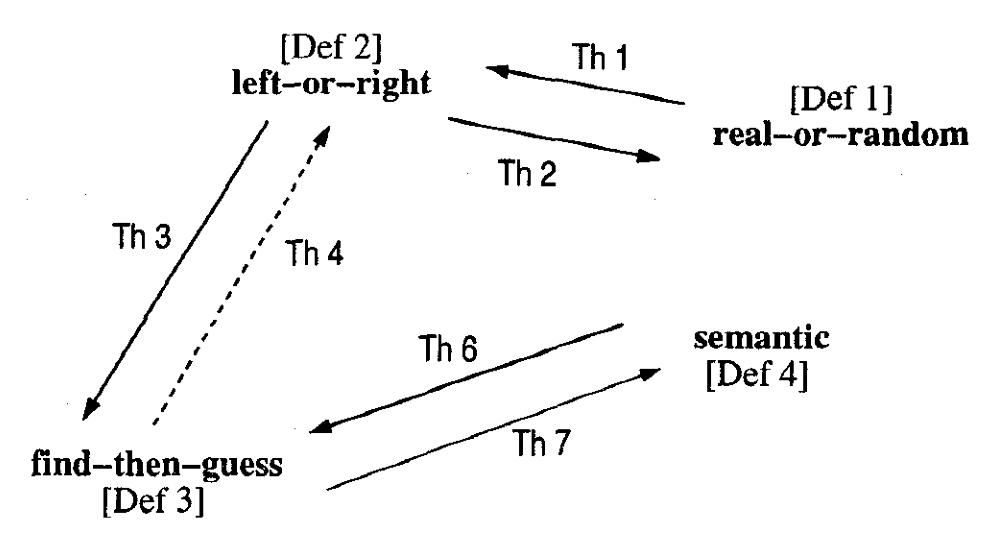
\includegraphics[width=0.8\textwidth]{Fig1.png}
	\caption{概念间的关系,从概念A到概念B的实线表示存在从A到B的安全性保持规约,A到B的虚线表示规约是安全性不保持的。}
	\label{Fig:fig1}
\end{figure}

虽然之前在方案分析的背景下考虑过具体安全性,但这是第一次考虑不同安全概念关系的工作。也就是说,这是第一次根据概念之间规约的复杂性将概念划分为较弱或较强。\par

实际上,这些结果很容易扩展到非对称方案。我们主要关注对称方案,因为这是我们要分析的方案所在的领域。

\subsection{加密方案的安全性}

我们分析了一些经典对称加密方案的安全性。具体来说,我们研究了使用分组密码(例如DES)的两种不同加密模式:CBC(密码块链接模式);和XOR(有时称为计数器模式)。对于后者,我们同时考虑概率和状态两种情况。\par

在这些方案中,底层本原(underlying primitive)\footnote{primitive有翻译为“原语”的,这里采用“本原”的翻译,保持了于冯登国老师在以下这篇文章中的翻译一致:冯登国. 可证明安全性理论与方法研究[J]. 软件学报, 2005, 16(10):14.}是伪随机函数(PRF)或伪随机置换(PRP)族F,
其中由密钥$a$指定的特定函数$F_a$将$l$比特映射到$L$比特,其中$l$和$L$是固定的(对于置换,$l=L$)。为了加密消息,$F_a$的应用以某种依赖于方案的方式迭代( iterated)\footnotemark。我们希望看到加密方案的安全性如何取决于PRF族的假定安全性。我们定义了PRF和PRP族的具体安全性,如[6]中所述,通过时间$t'$、Oracle查询数量$q'$和区分器(distinguisher)的最大优势$\epsilon'$的参数化。那么问题是:假设F是$(t',q';\epsilon')$安全($(t',q';\epsilon')-security$)的PRF族,那么$t,q,\mu,\epsilon$的值是什么,使得加密方案是$(t,q,\mu;\epsilon)$安全的?我们寻求上界和下界。(后者代表了最著名的攻击。)

\footnotetext{译者注:“以某种依赖于方案的方式迭代”的意思就是,用这个$F_a$采用不同的模式组成具体的加密方案,比如DES是可以采用不同模式形成不同的加密方案。这段话表明的意思是,一个基本元满足一个安全假设的前提下,用这些基本元进行组合时,安全性会一样吗?这个问题。}
\par

对于有状态XOR方案,我们证明了该方案对于$\epsilon =2 \epsilon ',\mu =q'l$和t与t’仅相差一个加法量 是 $(t,q,\mu;\epsilon)$安全的,这意味着该方案与我们可能希望得到的方案一样好。对于概率XOR方案,我们证明了该方案对于$\epsilon =2 \epsilon '+\mu (q-1)/(L2^l),\mu =q'l$
和t与前面描述一致的情况下是$(t,q,\mu;\epsilon)$安全。对于CBC,参数值是$\epsilon=2\epsilon '+(\mu^2 - \mu l)/(l^22^l),\mu=q' l$。在所有情况下,我们证明这些结果是严格的(tight),直到一个常数。我们得出结论,基于有限PRF的有状态XOR具有最佳安全性。
\par

上面所说的安全性是在“左或右不可区分”意义上的。根据我们之前所说的,这给出了其他三个概念一个可以比较的边界。

\subsection{更多历史}

我们已经提到了最重要的相关工作,即[11]。这里我们提供了一些更详细的比较和历史,并讨论了其他工作。\par

我们的结果表明,我们所考虑的概念在多项式时间规约下是等价的,因此可以在一个层面上将其视为对称情况下的[11]的模拟(analogue)。\par

在讨论不对称方案时,文章[8]表示对称方案可以类似地处理。这种观点中缺少的一个要素是,为了模型化选择明文攻击,必须在对称方案中为敌手提供某种加密手段。我们通过向对手提供加密预言(encryption oracle)来扩展多项式和语义安全。\par

也出现了比[11,17]更强的非对称加密概念,包括[19,7],但我们的关注仅限于在选择的明文攻击下保护隐私。\par

Luby[15]定义了对称加密的“发现-猜测安全”本质上是什么,他提到了使用伪随机函数族的加密,其输出长度是您希望加密内容的比特位数。他的处理方法对规约效率给予了一定的关注(尽管他并不像我们一样关注具体安全性)。\par

奇怪的是,一些早期的工作有一个更具体的处理方法:在非对称加密领域,Alexi等人[1]仔细地表明了其规约的复杂度,但后来许多工作不幸放弃了这一习惯。\par

从单向函数构造伪随机发生器[13]为从单向函数开始的对称加密提供了解决方案。在目前的工作中,存在不是问题\footnote{译者注:这句话的意思应该是“前面那种方案的存在不是问题”。};我们感兴趣的是具体安全性和对某些特定方案的分析。\par

[6]中提供了CBC MAC的具体安全性分析。(CBC MAC不应与CBC加密混淆:前者是消息身份验证代码。)我们基于他们的技术,但这些技术并不能直接解决这里的问题。CBC模式加密在[2,14,18]中标准化。

\subsection{关于此摘要文章}
本文一个扩展摘要,仅包含定义、方案描述和结果陈述。由于篇幅限制,证明被省略。我们论文的完整版本,包括所有证明,可以在[4]中找到。

\section{加密的概念}
对于所有复杂度度量,修复一些概率RAM模型(For all complexity measures fix some probabilistic RAM
model.)\footnote{译者注:这里的RAM模型就是计算复杂性里的RAM 计算模型。}。我们采用的约定是“时间”是指实际运行时间加上代码大小(相对于某些固定编程语言)。Oracle查询以单位时间回答。\par

如果$A(.,.,...)$是任何概率算法,则$a\leftarrow A(x_1,x_2,...)$表示在输入$x_1,x_2$上运行A的实验,并将$a$作为输出,概率是A的投币概率(the probability being over the coins of A.)。类似地,如果A是集合,则$a\leftarrow A$表示从A中均匀选择点并分配该值的实验。

\subsection{加密方案的语法}
将这些硬币(Coins)记为$\{0,1\}^\infty$(无限字符串的集合),设$MsgSp\subseteq \{0,1\}^*$是集合,消息空间,其中$x\in MsgSp$ 意味着每个与$x$具有相同长度的字符串$x'$,有$x'\in MsgSp$, 设$KeySp\subseteq \{0,1\}^*$是集合,表示密钥空间, 设$CipherSp=\{0,l\}^*$。
\par

 \textbf{\large{无状态加密(STATELESS ENCRYPTION).}} 一个(概率,无状态,对称)加密方案是一个三元组$\Pi=(\varepsilon,D,K)$:\par
 
$\varepsilon : KeySp\times MsgSp \times Coins\rightarrow CipherSp$\par
$D : KeySp\times CipherSp \rightarrow MsgSp$\par
$K :  Coins\rightarrow KeySp$\par

算法$\varepsilon$称为加密算法;$D$是解密算法;$K$是密钥生成器:我们要求对于所有$a\in KeySp$,$x\in MsgSp$,$r\in Coins$,有$D(a,\varepsilon(a,x,r))=x$。我们通常将第一个参数即密钥作为下标写入$\varepsilon$和$D$。我们称$\varepsilon_a(x,r)$为密钥$a$和硬币$r$下明文$x$的加密,或者更简洁地称为密文。我们将$D_a(y)$称为密钥$a$下密文$y$的解密。通常我们忽略了自变量$K$,将$K$视为概率算法,或是诱导概率空间(induced probability space)\footnotemark。类似地,我们经常忽略$\varepsilon$的最终参数,将$\varepsilon_a$视为概率算法,或将$\varepsilon_a(x)$视为诱导概率空间。在$y$不是密钥$a$下的任何字符串$x$的密文的情况下,记为$D_a(y)=\perp$。

\footnotetext{译者注:Given $(\Omega,\mathcal{A},\mathbb{P})$,It might be simpler to explain induced probability  with an example. Let $\Omega=\mathbb{R},\Omega′=\{0,1\}$ and $\mathbb{P}=N(0,1)$, that is
	\[\mathbb{P}=\frac{1}{\sqrt{2\pi}} \int_{A} e^{-\frac{x^2}{2}} dx\]
	for $A \in \mathcal{A}$, where $\mathcal{A}$ is the borel $\delta$-algebra on $\mathbb{R}$. To construct a Bernoulli variable we can consider $X: \Omega \rightarrow \Omega'$ as
	\[X(w)=\left\{
	\begin{aligned}
	1,w>0 \\
	0,w\leq 0
	\end{aligned}
	\right.
	\]
	We can now compute the induced measure on $\Omega'$, which will then be
	\[ \mathbb{P}=\mathbb{P}(\{w\in\Omega:w\leq 0\}) = \frac{1}{\sqrt{2\pi}} \int_{-\infty}^{0} e^{-\frac{x^2}{2}} dx    \]
	and similarly $\mathbb{P}(X^{-1}(\{1\}))=\dfrac{1}{2}$. We may thus conclude that X has a Bernoulli($\dfrac{1}{2}$) distribution, since that is the distribution that it induces. In fact you may take it as a definition, that the distribution of a random variable $X$ is the measure $\mathbb{P}_X$ that it induces.(from: https://math.stackexchange.com/questions/4309118/induced-probability-random-variable)
}
\par

对于一个有用的加密方案,$\varepsilon,D,K$应该是可有效计算的函数,但安全性的概念在这方面没有正式要求(formal demands,也可译为“形式化要求”)。\par

 \textbf{\large{有状态加密(STATEFUL ENCRYPTION).}}
 我们还考虑有状态加密方案,其中密文是一些信息的函数,如计数器,由加密方维护,并随每次加密而更新。在形式上,这种方案与之前的方案具有相同的语法,除了
 \[\varepsilon:KeySp \times MsgSp \times St \times Coins\rightarrow St \times CipherSp,\]
此处$St\subseteq \{0,1\}^*$是一组可能的状态,包含一个可区分的状态,空字符串$\epsilon$,我们称之为初始状态。设$\varepsilon^i(i=1,2)$表示$\varepsilon$的第i个分量。密文现在是(输出)$\varepsilon^2$,而$\varepsilon^1$是更新状态,由发送方存储,并用作加密函数下一次应用的第三个参数\footnote{译者注:也就是$St$}。请注意,加密变为有状态,但解密不会。
\par

\subsection{四个安全概念}
我们现在给出了四个安全概念,每个概念都模拟了选择明文攻击。在每种情况下,我们都允许对手以某种形式访问加密Oracle;这是这些定义区别于以前定义的一个特征。我们将描述无状态加密方案的定义,并在后面说明如何为有状态加密方案修改它们。
\footnote{译者注:原文以下内容并无标号,只是字体加粗大写,此处为了便于阅读将其排版为三级带标号标题。}
\par

\subsubsection{真实或随机(REAL-OR-RANDOM)}

其思想是,敌手无法区分文本加密和等长垃圾字符串加密。(通过传递性,敌手无法区分任何两个等长字符串的加密。)形式化考虑了两个不同的游戏。在游戏1中,我们首先选择一个随机密钥$a\leftarrow K$。然后给敌手一个Oracle,当向此Oracle询问字符串$x\in MsgSp$时,该Oracle用密钥a下的x(随机)加密进行响应。在游戏2中,我们开始选择随机密钥$a\in K$,然后,给对手一个Oracle,当向此Oracle询问字符串$x\in MsgSp$时,Oracle用它用长度为$|x|$的随机字符串的(随机)加密(在密钥a下)进行响应。如果没有“公平(reasonable)”敌手在区分游戏1和游戏2中获得“显著”优势,则加密方案是“好的”。\par

\begin{definition}[真实或随机(REAL-OR-RANDOM)]
	我们说加密方案$\Pi =(\varepsilon,D,K)$在“真实或随机”意义( real-or-random sense)上是$(t,q,\mu;\epsilon)$安全,当以下条件成立:
	\[Adv_A^{rr} \stackrel{def}{=} Pr[a\leftarrow K:A^{\varepsilon_a(\cdot)}=1] - Pr[a\leftarrow K : A^{\varepsilon_a(\$|\cdot|)}=1]\]
	$Adv_A^{rr} \leq \epsilon$,对于任意敌手A,其运行的时间最多为t,询问Oracle最多q次,这些总计最多为$\mu$比特。
\end{definition}

$A^{\varepsilon_a(\cdot)}$表示$A$有一个Oracle,A向此Oracle查询$x$,Oracle返回$y\leftarrow \varepsilon_a(x)$.(这意味着它选择一个随机字符串$r$并返回$\varepsilon_a (x,r)$,每次调用Oracle时都会选择一个新的随机字符串。)$A^{\varepsilon_a(\$|\cdot|)}$表示$A$有一个Oracle,A向此Oracle查询$x$,Oracle先选择$x'\leftarrow \{0,1\}^{|x|}$,然后返回$y\leftarrow \varepsilon_a(x')$做为响应.
\footnote{译者注:此定义表明两种不同Oracle都返回1的概率之差小于$\epsilon$。}

\subsubsection{左或右(LEFT-OR-RIGHT)}
我们再次考虑两个不同的游戏。在这两种游戏中,查询都是来自MsgSp的等长字符串对$(x_1,x_2)$。在任一游戏中,我们首先选择一个随机密钥$a\leftarrow K$,并在游戏期间固定该键,在游戏1中,一个Oracle接收$(x_1,x_2)$用来自$\varepsilon_a(x_1)$的随机样本进行响应。在游戏2中,它使用来自$\varepsilon_a(x_2)$的随机样本进行响应。因此,游戏1提供了“左”Oracle,而游戏2提供了“右”Oracle。如果“公平”敌手无法在区分游戏1和游戏2时获得“显著”优势,我们认为加密方案是“好的”。

\begin{definition}[左或右(Left-or-Right)]
	我们说加密方案$\Pi =(\varepsilon,D,K)$在“左或右”意义( Left-or-Right sense)上是$(t,q,\mu;\epsilon)$安全,如果对于任意敌手$A$,其运行的时间最多为t,询问Oracle最多q次,这些总计最多为$\mu$比特,且:
	\[Adv_A^{lr} \stackrel{def}{=} Pr[a\leftarrow K:A^{\varepsilon_a(left(\cdot,\cdot))}=1] - Pr[a\leftarrow K : A^{\varepsilon_a(right(\cdot,\cdot))}=1]\]
	$Adv_A^{lr} \leq \epsilon$。
\end{definition}
$A^{\varepsilon_a(left(\cdot,\cdot))}$表示$A$有一个Oracle,返回$y\leftarrow \varepsilon_a(x_1)$做为查询$(x_1,x_2)$的响应。
$A^{\varepsilon_a(right(\cdot,\cdot))}$表示$A$有一个Oracle,返回$y\leftarrow \varepsilon_a(x_x)$做为查询$(x_1,x_2)$的响应。

\subsubsection{查找-猜测(FIND-THEN-GUESS)}
这是对[ll,17]中给出的多项式安全概念的调整,我们想象一个分两个阶段运行的对手A,在敌手的“查找阶段(find stage)”,她努力想出一对长度相等的消息$x_0,x_1$,她想尝试区分它们对应的密码。她还保留了一些状态信息s,以便以后可能帮助她。在敌手的“猜测阶段(guess stage)”,她获得了一个明文$x_0$或$x_1$的随机密文$y$\footnote{译者注:这里随机的意思是“$x_0$和$x_1$之间随机取一个加密”},以及状态信息s。如果敌手正确识别了哪个明文与y对应,则敌手“获胜”。如果“公平”的对手在一半以上的时间内不能明显获胜,则加密方案是“好的”。
\begin{definition}[查找-猜测(Find-then-Guess)]
	我们说加密方案$\Pi =(\varepsilon,D,K)$在“查找-猜测”意义上是$(t,q,\mu;\epsilon)$安全,如果:
	\[Adv_A^{lr} \stackrel{def}{=} 2\cdot Pr[a\leftarrow K;
	(x_0,x_1,s)\leftarrow A^{\varepsilon_a(\cdot)}(find);
	b\leftarrow\{0,1\};
	y\leftarrow \varepsilon_a(x_b):A^{\varepsilon_a(\cdot)}(guess,y,s)=b
	]-1\]
	对于任意敌手$A$,$Adv_A^{lr} \leq \epsilon$,其运行的时间最多为t,询问Oracle最多q次,这些总计最多为$\mu$比特。
\end{definition}

据了解,上述要求$|x_0|=|x_1|$,乘2和减1只是比例因子,使得数值0对应于无优势,数值1对应于完全优势(perfect advantage)。\par

\subsubsection{语义(SEMANTIC)}
Goldwasser和Micali[11]解释了语义安全,他们说,在给定密文的情况下,可以有效计算明文的任何内容也可以在没有密文的条件下计算。我们采用[11,17]对于对称方案的形式化,设$f:MsgSp\rightarrow \{0,1\}^*$是明文$x$的某个函数,该函数表示x的信息,x是敌手试图找出的(The function represents the information about x that the adversary is trying to figure out.)。赋予MsgSp概率分布,
更具体地说,对于任何整数m,消息空间上的m分布(m-distribution)是MsgSp上概率分布的集合$M=\{M_\gamma\}_{\gamma\in \{0,1\}^{\leq m}}$,由字符串$\gamma\in \{0,1\}^{\leq m}$索引。
我们假设每个分布都是有效的,这意味着对于所有$\gamma$,$M_\gamma$中所有非零概率的字符串都具有相同的长度,并且该长度最多为$m$。设$p_{f,M_\gamma}^* = max_{y^*}\{Pr[x\leftarrow M_\gamma : f(x)=y^*]\}$,这是最可能的$f(\cdot)$值的概率。


我们的敌手将分为两个阶段。在敌手的选择阶段,它努力提出有利的分布$M_\gamma$。在对手的预测阶段,根据分布$M_\gamma$选择的明文x给出随机密文y,并希望猜测$f(x)$。如果没有公平敌手A能够以显著优于$p^*_{f,M_\gamma}$的概率猜测$f(x)$,则加密方案对于函数$f$和分布$M$是语义安全的。


先前的形式化要求所有函数f此条件成立,在我们的具体处理中,函数$f$和概率分布$M$都成为参数,因此我们可以测量明文的特定属性在特定分布下受到保护的程度。


\begin{definition}[语义(Semantic)]
	设$f: MsgSp \rightarrow \{0,1\}^*$是一个函数,$M=\{M_\gamma\}_{\gamma\in \{0,1\}^{\leq m}}$是一个在MsgSp上的m-分布,加密方案$\Pi =(\varepsilon,D,K)$在“语义”意义上是$(t,q,\mu;\epsilon)$安全,对于$M$上的$f$,如果\par
	\begin{align*}
		Adv^{sm}_A(f,M) \stackrel{def}{=} & E[a\leftarrow K;(\gamma,s)\leftarrow A^{\varepsilon_a(\cdot)}(select):\\
		 & \alpha (a,\gamma,s)]\leq \epsilon,	 where\\
		 \alpha (a,\gamma,s)=& Pr[x\leftarrow M_\gamma;y\leftarrow \varepsilon_a(x): \\
		                     & A^{\varepsilon_a(\cdot)}(predict,y,s)=f(x)]-p^*_{f,M_\gamma},
	\end{align*}
	对于任何敌手A,其运行的时间最多为t,询问Oracle最多q次,这些总计最多为$\mu$比特。		
\end{definition}

\subsubsection{为有状态案例修改定义}
有状态加密方案的安全定义是通过以自然方式修改上述定义,调整如何回答Oracle查询来获得。例如,在定义1中,
$A^{\varepsilon_a(\cdot)}$现在表示具有Oracle的$A$保持在状态$\delta$,初状态为$\epsilon$。在接收到查询$x$时,它选择硬币
$\gamma$,并将$(\delta^{'},y)$设置为$\varepsilon_a(x,\delta,\gamma)$。它返回$y$作为Oracle查询的答案,并通过$\delta \leftarrow \delta^{'}$更新状态。请注意,返回了密文(就是$y$),但更新的状态不是。(因此,我们在写$A^{\varepsilon_a(\cdot)}$时是滥用了符号;我们应该编写$A^{\varepsilon^2_a(\cdot)}$。)请注意,加密Oracle现在有“内存”:在调用之间,状态被修改和保留。符号$A^{\varepsilon_a(\textdollar|\cdot|)}$可以类似地重新解释,同样的方法适用于其他三个定义。

\subsubsection{渐进定义(ASYMPTOTIC DEFINITIONS)}
我们的定义很容易扩展到标准渐近框架,简单地说,方案在给定意义上是安全的,如果作为方案依赖的基础安全参数的函数对于任何多项式时间敌手的优势可以忽略。(Our definitions are easily extended to the standard asymptotic framework by simply saying that a scheme is secure, in a given sense, if the advantage of any polynomial time adversary is negligible, as a function of an underlying security parameter on which the scheme now depends.)上述公式只是使我们能够作出更具体的陈述。

\section{概念间规约}
在这里,我们看看不同安全概念之间的规约。我们同时考虑上界和下界。这些结果的证明在[4]中。

因为我们关注的是具体的安全边界,所以我们可以使用我们的结果来确定相对于多项式等价的其他概念,安全性的作用有多强。这一信息很有用,因为它有助于我们确定最理想的削减起点。当我们通过从左或右不可区分性的规约来证明方案的安全性时,我们在第4节中隐含地使用了这一信息。

在下面的定理中,$c$是一个绝对常数,仅取决于基础计算模型的细节。前两个定理表明,我们的前两个概念,左或右不可区分性和实或随机不可区分,本质上是等价的。

\begin{theorem}[“实或随机”意味着“左或右”]
	对于常数$c>0$,如果加密方案$\Pi=(\varepsilon,D,K)$在“实或随机”意义上是$(t_1,q_1,\mu_1;\epsilon_1)-secure$,那么此方案在“左或右”意义上是$(t_2,q_2,\mu_2;\epsilon_2)-secure$,此处$t_2=t_1-c\cdot \mu_2,q_2=q_1,\mu_2=\mu_1,\epsilon_2=2\epsilon_1$。
\end{theorem}

\begin{theorem}[“左或右”意味着“实或随机”]
	对于常数$c>0$,如果加密方案$\Pi=(\varepsilon,D,K)$在“左或右”意义上是$(t_2,q_2,\mu_2;\epsilon_2)-secure$,那么此方案在“实或随机”意义上是$(t_1,q_1,\mu_1;\epsilon_1)-secure$,此处$t_1=t_2-c\cdot \mu_1,q_1=q_2,\mu_1=\mu_2,\epsilon_1=\epsilon_2$。
\end{theorem}

左或右不可区分性和真实或随机不可区别性构成了比传统的发现-猜测概念更强的安全概念。凭直觉,发现-猜测概念对对手来说更难,因为它必须挑选出一个消息对来执行。定理3和4以及命题5说明了这一点。

第一个定理说\footnote{译者注:这里觉得应该是原作者的一个笔误,应该是下一个定理。},在左或右意义上具有一定安全性的方案在查找-然后猜测意义上基本上具有相同的安全性。

\begin{theorem}[“左或右”意味着“查找-猜测”]
	对于常数$c>0$,如果加密方案$\Pi=(\varepsilon,D,K)$在“左或右”意义上是$(t_2,q_2,\mu_2;\epsilon_2)-secure$,那么此方案在“查找-猜测”意义上是$(t_3,q_3,\mu_3;\epsilon_3)-secure$,此处$t_3=t_2-c\cdot \mu_3,q_3=q_2,\mu_3=\mu_2,\epsilon_3=\epsilon_2$。
\end{theorem}

下一个定理说,如果一个方案在查找-猜测意义上具有一定的安全性,那么它在左或右意义上是安全的,但所示的安全性在数量上较低。

\begin{theorem}[“查找-猜测”意味着“左或右”]
	对于常数$c>0$,如果加密方案$\Pi=(\varepsilon,D,K)$在“查找-猜测”意义上是$(t_3,q_3,\mu_3;\epsilon_3)-secure$,那么此方案在“左或右”意义上是$(t_2,q_2,\mu_2;\epsilon_2)-secure$,此处$t_2=t_3-c\cdot \mu_2,q_2=q_3,\mu_2=\mu_3,\epsilon_2=q_2 \epsilon_3$。
\end{theorem}

下面的命题表示,上述安全性的下降不是由于规约中的任何弱点,而是内在的——我们提出了一个方案,在“查找-猜测”的意义上比在左或右的意义上具有更高的安全性,间隙与上述定理相同。显然,如果周围根本没有安全加密方案,我们就不能做出这样的声明,因此定理假设存在一个安全方案,然后构造一个显示所需间隙的不同方案。

在下文中,将$\epsilon'$视为非常小(基本上为零)。构造的方案$\Pi'$可以用概率$\epsilon_2=0.632$在左或右意义上使用$q$查询破解,这意味着在这个概念下它是完全不安全的。然而,在“查找-猜测”的意义上,破解它(具有可比资源)的概率是$\epsilon_3\approx \dfrac{1}{q}$。概率服从关系式$q\epsilon_3 = \Theta(\epsilon_2)$,表明定理4本质上是严格的。此外,如果允许方案是有状态的,则可以使$\epsilon_2$恰好为1,因此$q\epsilon_3 \approx \epsilon_2$。

\begin{proposition}["左或右"比"查找-猜测"强]
	常数$c>0$,并且下面描述为真,假定在包含$\{0,1\}$的消息空间上存在一个无状态加密方案,并且是“查找-猜测”意思上的$(t',q,\mu;\epsilon')-secure$,那么这里存在一个无状态加密方案$\Pi'$,其在“左或右”意义上是$(t_2,q,q;\epsilon_2)-breakable$($(t_2,q,q;\epsilon_2)$可破解),在“查找-猜测”意义上是$(t_3,q,\mu;\epsilon_3)-secure$,此处$\epsilon_2=0.632,\epsilon_3=\epsilon'+\dfrac{1}{q}$,并且,$t_2=cq,t_3=t'$。进一步,这里存在一个有状态加密方案$\Pi^{''}$,此方案有同样的特征,除去$\epsilon_2=1$.
\end{proposition}

语义安全性太复杂,无法作为证明方案安全性的良好起点。尽管如此,正如下一个定理所指出的,语义安全性到查找-猜测安全有一个很强规约。请注意,这只需要特定的简单函数、标识函数以及消息空间上的特定简单分布保持语义安全性。对于非对称加密方案,该定理在[11]中是隐式的,并且它们的证明很容易适用于对称设置。

\begin{theorem}[语义包含“查找-猜测”]
	设$f$是恒等函数(identity function)\footnote{译者注:恒等函数是指$f(x)=x$.},对于任意在MsgSp空间上具有相同长度的字符串对$r=(x_0,x_1)$,设$M_r$是对每个$x_0,x_1$概率是1/2,对于所有其他字符串概率为0的分布,当$r$不具有这种形式时,$M_r$是任意定义的。设$M=\{M_r\}_{r\in \{0,1\}\leq t_4}$,那么对于某个常数$c>0$,如果$\Pi$在语义意义上对于$M$上的所有$f$是$(t_4,q_4,\mu_4;\epsilon_4)-secure$,那么此方案在“查找-猜测”意义上是$(t_3,q_3,\mu_3;\epsilon_3)-secure$,此处$t_3=t_4-c\cdot \mu_3,q_3=q_4,\mu_3=\mu_4,\epsilon_3=2\epsilon_4$.
\end{theorem}

将其与定理4相结合,产生了从语义意义上的安全性到左或右意义上的的安全性的规约,但这种规约继承了定理4规约的安全性损失。如前所述,证明这种损失是固有的:左或右的安全性是一个更强的概念。看到这一点的示例与命题5的证明基本相同,但设置变得更加复杂。我们在此不再进一步讨论。

在另一个方向上,对消息空间进行采样和计算函数$f$的时间复杂度也会出现。设$T_M(\cdot)$是一个函数,将$|r|$作为输入,并从$M$返回采样时间的边界。设$T_f(\cdot)$表示计算给定$x$的$f(x)$的时间,用$|x|$的函数来度量。假设两个时间函数都是单调的。

\begin{theorem}[“查找-猜测”包含语义]
	有一个常数$c>0$以下为真。$f$是一个函数,其计算时间为$T_f(\cdot)$,设$M$是一个在MsgSp上有效的m分布,可在时间$T_M(\cdot)$内采样,如果$\Pi=(\varepsilon,D,K)$在"查找-猜测"意义上是$(t_3,q_3,\mu_3;\epsilon_3)-secure$,那么其在$M$上的$f$语义意义上是$(t_4,q_4,\mu_4;\epsilon_4)-secure$,此处$t_4=t_3-2T_M(m)-T_f(m)-c\cdot \mu_4,q_4=q_3,\mu_4=\mu_3,\epsilon_4=2\epsilon_3$.
\end{theorem}

注意,函数$T_M(\cdot),T_f(\cdot)$越大,定理7给出的$M$上$f$的语义安全性越低。这反映了现实吗?也就是说,我们是否会期望对手比计算明文的简单属性更容易计算明文的复杂属性?可能在任何情况下,当信息函数$f$很简单时,这些定理最有用,就像所有位的异或。

在早期的工作[11,17,8]中,对$f$的复杂性没有任何限制,甚至允许它是不可计算的。很明显,针对这种非常复杂的函数的语义安全性并不遵循定理7。然而,似乎可以使用[8]的技术进行不同的规约。这里,$f$的复杂性不会进入(尽管采样$M_r$的复杂性仍然重要)。对其他参数的依赖性将增加。因此,该定理在讨论复杂函数$f$时有用,但在讨论简单函数时不如定理7有用。我们目前没有更多地追求这一点,因为正如我们上面所指出的,其他安全概念比语义安全更适合作为实际方案要满足的目标。

将这些东西放在一起,显示加密方案左或右安全或实或随机安全意味着对所有其他概念的严格简化(对语义安全的f和M复杂性的技术限制进行模)。显示加密方案“查找-猜测”安全或语义安全不安全。因此,如果边界相等,最好证明前两个概念之一的安全性,因为这会立即转化为其他概念的相同良好边界。

\section{方案分析}

接下来,我们将分析对称加密的方案。所有这些方案都基于有限伪随机函数,这是[6]引入的伪随机函数[10]原始概念的具体安全版本。因此,在后一篇文章之后,我们从一些必要的定义开始。本节给出的结果证明见[4]。

\subsection{有限PRFs和PRPs}
函数族是函数F的多个集合,其中F中的所有函数具有相同的域和范围。通常,域是$\{0,l\}^l$,范围是$\{0,l\}^L$,分别称为输入长度$l$和输出长度$L$。我们假设集合$K$中的每个密钥$a$指定$F$中的函数$F_a:\{0,1\}^l \rightarrow \{0,1\}^L$。通常,$K$是某个固定长度$k$的所有字符串的集合。我们用$f\leftarrow F$表示通过随机选择$a\leftarrow K$从$F$中随机选取一个函数的操作,$f=F_a$。

对于应用程序可访问的函数族$F$,我们通常希望在给定$a$的情况下,可以容易地计算$F_a$。但我们在这方面没有形式化要求(formal requirements),实际上,考虑“不可访问”函数族(“inaccessible” function families)是有用的,如下所示。

设$R_{l,L}$是由从$l$位长度字符串集合到$L$比特字符串长度集合的所有函数组成的函数族。(密钥$a$可以被视为函数的完整描述。)理解了$l,L$,我们写R而不是$R_{l,L}$。因此,$f\leftarrow R$是随机从$l$个比特到$L$个比特函数选择的操作。类似地,我们让$P_l$是由$1$比特字符串上的所有置换组成的函数族。理解了$1$,我们$P_l$简写为$P$。

设$F,G$是具有相同输入和输出长度的函数族。考虑一种被称为区分器(distinguisher)的Oracle算法,该算法试图区分Oracle h从$F$中随机选择的情况和h从$G$中随机选择。设$Dist_D(F,G)=Pr[h\leftarrow F:D^{h(\cdot)=1}]-Pr[h\leftarrow G:D^{h(\cdot)}]=1$.\footnote{译者注:公式中的Dist表示distinguisher}
伪随机函数族具有这样一个性质,对于不知道随机选择的密钥a的人来说,F的输入输出行为“看起来随机”。“看起来随机”有两个重要的概念。第一个看起来像一个随机函数(random function),第二个看起来像是一个随机排列(random permutation)。因此,我们定义$Adv_D^{rf}(F)=Dist_D(F,R)  and  Adv_D^{rp}(F)=Dist_D(F,P)$。\footnote{译者注:rf表示random function,rp表示random permutation}


\begin{definition}[PRF/PRP族的具体安全,[6]]
	函数族F被称为$(t,q;\epsilon)$安全PRF(PRP同样)族,如果对于进行最多$q$个Oracle查询并在最多$t$时间内运行的任何区分器$D$,我们有$Adv_D^{rf}(F)<\epsilon$(同样有$Adv_D^{rp}(F)<\epsilon$)。
\end{definition}

注意,与Luby和Rackoff[16]不同,我们通过到随机置换族的距离来衡量PRP族的质量,而不是随机函数。这是因为我们定义的PRP族是比PRF族更好的分组密码模型,如DES。(当然,区别仅在于具体的安全,但这确实是我们关注的问题。)然而,这两个概念之间的以下关系通常就足够了:

\begin{proposition}[PRP族就是PRF族]\label{proPRP_PRF}
	假定$F$是$(t,q;\epsilon)$安全的PRP族,输入和输出长度都是$l$,那么$F$是$(t,q;\epsilon')$安全的PRF族,此处$\epsilon' =\epsilon -q^2 2^{-l-1}$.
\end{proposition}

特定分组密码的估计的密码分析强度为我们提供了$t,q,\epsilon$值的估计,特定分组密码(如DES)可被视为$(t,q;\epsilon)$安全的PRP族。上述命题给了边界,通过这个定理我们可以将其视为$(t,q;\epsilon)$安全的PRF。

\subsection{XOR方案}
固定输入长度为$1$、输出长度为$L$和密钥长度为$k$的函数族F。我们让$a$表示运行加密方案的双方之间共享的密钥。它将用于指定函数$f=F_a$。事实上,所有的方案都只依赖于这个函数,也就是说,它们可以在给定函数的Oracle的情况下实现。我们设$R=R_{l,L}$。

XOR模式有两个版本:无状态(随机)和有状态(基于计数器和确定性)。

\textbf{{\large 说明(Specifications).}}  方案$XOR\textdollar(F)=(\varepsilon-XOR\textdollar,D-XOR\textdollar,K-XOR\textdollar)$ 工作过程如下。密钥生产算法$K-XOR\textdollar$为基础PRF族F输出一个随机$k$比特密钥$a$,从而确定一个从$l$比特映射到$L$比特的函数$f=F_a$,消息$x$的加密看作是一个$L$比特块序列(如果需要首先要填充),$x=x_1\cdots x_n$。我们定义$\varepsilon-XOR\textdollar_a(x) = \varepsilon-XOR\textdollar^{F_a}(x)$,$D-XOR\textdollar_a(z) = D-XOR\textdollar^{F_a}(z)$,下面定义:\\
\textbf{function} $\varepsilon-XOR\textdollar^f(x)$\\
(1)$r\leftarrow \{0,1\}^l$\\
(2)for $i=1,\cdots,n$ do $y_i=f(r+i)\oplus x_i$\\
(3)return $r\parallel y_1y_2\cdots y_n$\\
\textbf{function} $D-XOR\textdollar^f(z)$\\
(1) Parse $z$ as $r \parallel y_1\cdots y_n$\\
(2) for $i=1,\cdots,n$ do $x_i=f(r+i)\oplus y_i$\\
(3) return $x=x_1\cdots x_n$\\
我们称$r$为nonce,上面的加法是模$2^l$,并且在通常情况下,结果也被编码为一个$l$比特串。

这个方案也有一个有状态的变种,$XORC = (\varepsilon-XORC,D-XORC,K-XORC)$,此处$r$扮演的角色是一个$l$比特计数器,记为$ctr$,初始为$-1$,每次加密后增加加密块的数量。注意,只有发送方维护计数器,并将其作为密文的一部分输出,对方案的限制是加密块的总数最多为$2^l$。

密钥生产算法$K-XORC$与前面定义相同,为PRF族输出一个随机密钥$a$,使用与上述相同的格式约定,我们定义$\varepsilon-XORC_a(x,ctr)=\varepsilon-XORC^{F_a}(x,ctr)$和$D-XORC_a(z)=D-XORC^{F_a}(z)$,此处:\\
\textbf{function} $\varepsilon-XORC^f(x,ctr)$\\
(1)for $i=1,\cdots,n$ do $y_i=f(ctr+i)\oplus x_i$ \\
(2)$ctr\leftarrow ctr+n$ \\
(3)return ($ctr,ctr\parallel y_1y_2\cdots y_n$)\\
\textbf{function} $D-XORC^f(z)$\footnote{译者注:此处原文为$D-XOR\textdollar^f(z)$,应该是作者笔误,翻译是改为$D-XORC^f(z)$}\\
(1) Parse $z$ as $ctr \parallel y_1\cdots y_n$\\
(2) for $i=1,\cdots,n$ do $x_i=f(ctr+i)\oplus y_i$\\
(3) return $x=x_1\cdots x_n$\\


\textbf{{\large 方案特点(FEATURES OF THE SCHEMES).}}   请注意,解密不需要$f=F_a$的逆,因此$F_a$不需要是置换。

与更常见的操作模式相比,XOR方案具有一些计算优势。即,不同块上的$F_a$计算可以并行进行,因为一个块上的计算独立于其他块。这种并行性优势可以通过硬件或软件支持来实现。如果每个块都标记有其索引,则不必按顺序进行解密。这些方案还支持离线处理,即$F_a$计算可以在使用这些消息前的空闲时间内完成。

\textbf{{\large $XOR\textdollar$的安全性(SECURITY OF $XOR\textdollar$).}}   我们首先推导出了对手试图在左或右意义上破坏$XOR\textdollar(F)$方案的成功率的下界。在常见的密码术语中,这意味着我们正在提供攻击。我们指定的攻击是针对“理想”方案,即底层函数$f$是真正随机函数。

\begin{proposition}[在随机函数模型下$XOR\textdollar$的安全下界]\label{XORSECBOUNDS}
	这里有一个$XOR\textdollar(R_{l,L})$的敌手$E$,在左或右意义上,其最多可进行$q$个查询,总计最多$\mu$比特,($\mu q /L \leq 2^l$) 并且达到$Adv_E^{lr}\geq 0.316\cdot [\mu\cdot (q-1)]/[L\cdot 2^l]$.
\end{proposition}

这是一次“生日”攻击。如果我们让$\overline{n}=\mu / (Lq)$为每个查询的平均块数,则可能更容易测量,因此$\mu =Lq\cdot \overline{n}$。然后我们看到$Adv^{lr}_E = \Omega(q^2/2^l)\cdot \overline{n}$,这是典型的生日行为,表现出对查询数量的二次依赖。

由于我们在随机函数模型中证明了一个下界,因此我们不讨论$E$使用的时间。然而,从策略中可以清楚地看出,除了Oracle调用的时间之外,$E$使用的总时间只是一点点开销。所有下界都是如此,我们不再提及。

命题\ref{XORSECBOUNDS}指出,即使底层分组密码$F$非常好(它不能比真正的随机更好),$XOR$方案也会随着越来越多的数据被加密而泄漏一些信息。接下来,我们展示了上述基本上是最好的攻击:一个人不可能获得更好的优势,直到一个恒定的因素。下面的关键点是,边界对任何对手都适用。

\begin{lemma}[在随机函数模型中$XOR\textdollar$安全上界]
	设$E$是任意敌手在左或右意义上攻击$XOR\textdollar(R_{l,L})$,最多查询$q$次,合计最多$\mu$比特,那么$Adv^{lr}_E \leq \delta_{XOR\textdollar}=[\mu (q-1)]/[L\cdot 2^l]$.
\end{lemma}

当然,当我们使用分组密码时,理想模型中的安全性指示不是安全性指示。然而,“现实世界”的情况很容易从上面得到:

\begin{lemma}[使用为伪随机函数时$XOR\textdollar$安全]
	有一个常数$c>0$,以下为真。假定$F$是$(t',q';\epsilon')$安全的PRF族,输入长度$l$,输出长度$L$,那么对于任一个$q$,$XOR\textdollar$方案在左或右意义上是$(t,q;\epsilon)$安全,对于$\mu=q' L,t=t'-c\cdot \frac{\mu}{L}(l+L),\epsilon=2\epsilon'+\delta_{XOR\textdollar}$,此处$\delta_{XOR\textdollar}\stackrel{def}{=}[\mu(q-l)]/[L\cdot 2^l]$.
\end{lemma}

\textbf{{\large $XORC$的安全性(SECURITY OF $XORC$).}}  
该方案的有状态版本具有更好的安全性。在理想情况下,对手没有优势:

\begin{lemma}[随机函数模型中$XORC$安全上界]
	设$E$是任意敌手在左或右意义上攻击$XORC(R_{l,L})$,最多查询$q$次,合计最多$\mu< L2^l$比特,那么$Adv^{lr}_E =0$.
\end{lemma}

这个翻译为以下“真实世界”安全:

\begin{theorem}[使用伪随机函数的$XORC$安全]
	这里有个常数$c>0$,以下成立。假定$F$是$(t',q';\epsilon')$安全的PRF族,输入长度$l$,输出长度$L$,那么对于任一个$q$,$XORC(F)$方案在左或右意义上是$(t,q;\epsilon)$安全,对于$\mu=min(q' L,L2^l),t=t'-c\cdot(\mu/L)(l+L) ,\epsilon=2\epsilon'$.
\end{theorem}

\subsection{CBC方案}

对于CBC方案,我们要求$l=L$($F$的输入和输出长度相同),并且每个$F$都是一个置换,以便给定$a$,我们不仅可以计算$F_a$,还可以计算$F^{-1}_a$。然而,就安全性而言,我们仍然将$F$视为伪随机函数族。在说明了本案例的结果之后,我们将讨论当$F$是PRP家族时会发生什么。

\textbf{{\large 说明(Specifications).}}  方案$CBC\textdollar(F)=(\varepsilon-CBC\textdollar,D-CBC\textdollar,K-CBC\textdollar)$与前面的方案有相同的密钥生成算法,这意味这加密密钥a确定了$f=F_a$,被加密的消息$x$可以看成一个$l$比特大小的块组成的序列,$x=x_1\cdots x_n$,我们定义$\varepsilon-CBC\textdollar_a(x)=\varepsilon-CBC\textdollar^{F_a}(x)$和$D-CBC\textdollar_a(z)=D-CBC\textdollar^{F_a}(z)$,此处:\\
\textbf{function} $\varepsilon-CBC\textdollar^f(x)$\\
(1)$y_0\leftarrow \{0,1\}^l$\\
(2)for $i=1,\cdots,n$ do $y_i=f(y_{i-1})\oplus x_i$\\
(3)return $y_0\parallel y_1y_2\cdots y_n$\\
\textbf{function} $D-CBC\textdollar^f(z)$\\
(1) Parse $z$ as $y_0 \parallel y_1\cdots y_n$\\
(2) for $i=1,\cdots,n$ do $x_i=f^{-1}(y_i)\oplus y_{i-1}$\\
(3) return $x=x_1\cdots x_n$\\
$y_0$的值被称为初始向量或nonce,下面是对计数器变种的讨论。

\textbf{{\large $CBC\textdollar$的安全}}  甚至当底层块加密是理想的时候,生日攻击依然可能。

\begin{proposition}[在随机函数模型中$CBC\textdollar$安全下限]\label{lb_CBC_RFM}
	$CBC\textdollar(R_{l,L})$在左或右的意义上有一个对手$E$,他最多进行$q$个查询,总计最多$\mu$比特($\mu \leq l\cdot 2^{l/2}$),并达到:
	\[Adv^{lr}_{E} \geq 0.316\cdot (1-2\cdot 2^{-l/2})\cdot (\frac{\mu ^2}{l^2}-\frac{\mu}{l})\cdot \frac{1}{2^l}.\]
\end{proposition}

然而,这些是在恒定因素下可能的最佳攻击:

\begin{lemma}[在随机函数模型中$CBC\textdollar$安全上限]\label{ub_CBC_RFM}
	$CBC\textdollar(R_{l,L})$在左或右的意义上有一个对手$E$,他最多进行$q$个查询,总计最多$\mu$比特,那么有:
	\[Adv^{lr}_{E} \leq \delta_{CBC\textdollar} \stackrel{def}{=}(\frac{\mu ^2}{l^2}-\frac{\mu}{l})\cdot 2^l.\]
\end{lemma}

“现实世界”安全如下:

\begin{theorem}[使用伪随机函数的$CBC\textdollar$的安全]\label{CBC_PF}
	存在一个常数$c>0$使得以下关系成立。假定$F$是输入长度为$l$,输出长度为$L$的$(t',q';\epsilon')$安全的PRF族,那么对于任意$q$,$CBC\textdollar(F)$在左或右意义上是$(t,q,\mu;\epsilon)$安全,$\mu=q'l,t=t'-c\mu,\epsilon=2\epsilon'+\delta_{CBC\textdollar}$,此处$\delta_{CBC\textdollar}\stackrel{def}{=}(\frac{\mu^2}{l^2}-\frac{\mu}{l})\cdot 2^{-l}$.
\end{theorem}

假设$F$是一个PRP族,而不是PRF族,那么$CBC$确实应该被分析,因为该方案确实必须用置换,而不是函数。对于上界,它实际上没有什么区别,因为我们可以将命题\ref{proPRP_PRF}应用于引理\ref{ub_CBC_RFM}来进行翻译。然而,对于下限来说,这并没有帮助。因此,在这一点上,可以想象,如果$F$是PRP族,$CBC$加密比上界指示的安全得多。但事实上,这不是真的。如下所述,相同的下界适用于置换。

\begin{proposition}[在随机置换模型中$CBC\textdollar$安全下届]\label{lb_CBC_RPM}
		$CBC\textdollar(P_{l,L})$在左或右的意义上有一个对手$E$,他总计进行$\mu$比特查询(($\mu \leq l\cdot 2^{l/2}$)),达到:
		\[Adv^{lr}_{E} \geq 0.316\cdot (\frac{\mu ^2}{l^2}-\frac{\mu}{l})\cdot {2^l}.\]
\end{proposition}

注意,命题\ref{lb_CBC_RFM}适用于任何$q$。相反,在命题\ref{lb_CBC_RPM}中,给定$p$,我们允许对手选择一个方便的$q$(结果是$q=\mu/l$)。在这个意义上,命题\ref{lb_CBC_RPM}较弱。我们认为有可能改进命题\ref{lb_CBC_RPM},但目前尚未进行分析。

\textbf{{\large 有计数器的$CBC$(CBC WITH COUNTERS).}} 我们很容易做出$CBC$的计数器变体,并希望提高(或至少保持)安全性。实际上,在各种书籍中建议初始化向量可以是计数器。但这不起作用;知道计数器的下一个值后,对手可以选择一个消息查询,该查询将强制$f$的输入发生冲突,从而破坏方案(在任何定义下)。


为了制作$CBC\textdollar$的正确计数器版本,可以让初始化向量为$y_0=f(ctr)$,并在每次加密后将$ctr$递增1。该方案能够加密最多$2^l$条消息。因此,类似于定理\ref{CBC_PF}是可能的。如果用于确定$y_0$的密钥与用于$CBC$加密的其余部分的密钥分离,则结果最简单(作为定理16的推论)。

\section*{致谢}
我们感谢兰·卡内蒂(Ran Canetti),他对早期草案提出了一些有益的意见,并感谢吉姆·格雷(Jim Gray),他提出了此处出现的定义1的变体。

\section*{参考文献}
[l] W. ALEXI, B. CHOR, 0. GOLDREICH, C. SCHNORR,“RSA and Rabin functions: Certain parts are as hard as the
whole,” SIAMJoumal on Computing Vol. 17, No. 2, 1988,pp. 194-209.

[2] ANSI X3.106, “American National Standard for Information Systems - Data Encryption Algorithm -Modes of Operation,” American National Standards Institute, 1983.

[3] M. BELLARE, R. CANETTI AND H. KRAWCZYK “Psuedo-random functions revisited: The cascade construction and
its concrete security,” FOCS 96.

[4] M. BELLARE, A. DESAI, E. JOKIPII AND P. ROGAWAY, “A concrete security treatment of symmetric en-
cryption,” full version of this paper, available at http://www-cse.ucsd.edu/users/mihir.

[5] M. BELLARE, R. GUBRIN AND P. ROGAWAY, "XOR MACS: New methods for message authentication using finite pseudorandom functions,” Crypto 95.

[6] M. BELLARE, J. KILIAN AND P. ROGAWAY, ‘The security of cipher block chaining,” Crypto 94.

[7] D. DOLEV, C. DWORK AND M. NAOR, “Non-malleable cryptography,” STOC 91.

[8] O. GOLDREICH “A uniform complexity treatment of encryption and zero-knowledge,” Journal of Cryptology,
Vol. 6, 1993, pp. 21-53.

[9] O. GOLDREICH, R. IMPAGLIAZZO, L. LEVIN,R. VENKATESAN AND D. ZUCKERMAN, “Security preserving amplification of hardness,” FOCS 90.

[l0] O. GOLDREICH, s. GOLDWASSER AND s. MICALI, “How to construct random functions,” Journal of the ACM,
Vol. 33, No. 4, 1986, pp. 210-217.

[11] S. GOLDWASER AND s. MICALI, “Probabilistic encryption,” J. of Computer and System Sciences, Vol. 28,
April 1984, pp. 270-299.

[12] A. HERZBERG AND M. LUBY, “Public randomness in cryptography,” Crypto 92.

[13] J. HASTAD, R. IMPAGLIAZZO, L. LEVIN AND M. LUBY,“Construction of a pseudo-random generator from any one-
way function,” ICSI Technical Report, No. 91-068, submitted to SICOMP.

[14] IS0 8372, “Information processing - Modes of operation for a 64-bit block cipher algorithm,” International Organization for Standardization, Geneva, Switzerland, 1987.

[15] M. LUBY, Pseudorandomness and Cryptographic Applications, Princeton University Press, 1996.

[16] M. LUBY AND C . RACKOFF, “How to construct pseudorandom permutations from pseudorandom functions,”
SIAM J. Computation, Vol. 17, No. 2, April 1988.

[17] S . MICALI, c. RACKOFF AND R. SLOAN, “The notion of security for probabilistic cryptosystems,” SIAM J. of Com
puting, April 1988.

[18] National Bureau of Standards, NBS FIPS PUB 81, “DES modes of operation,” U.S Department of Commerce, 1980.

[19] M. NAOR AND M. YUNG, “Public-key cryptosystems provably secure against chosen ciphertext attacks,”
STOC 90.

[20] A. C. YAO, “Theory and applications of trapdoor functions,” FOCS 82.

\end{document}
